\section{Testing Environment}\label{sec:testing-environment}
This section will explain how the testing environment is setup and what tools have been used and configured.

\begin{itemize}
	\item Since performance is being tested, the result will vary depending on system. The system used is shown in Table~\ref{tab:test-system-specs}
    \item Docker is being used for creating disposable containers, the "Dockerfile's" and other configurations can be found in the project git repository, links can be found at Appendix~ \ref{project-links}
	\item Wireshark is being used to collect packets; statistics are exported as CSV from the "Statistics" tab using both "IO Graph" and "Conversations"
	\item To get accurate test results a mix of real and synthetic files are being used, these are documented in Table~\ref{tab:file-types-used-for-testing}
	\item The following data points will be collected
	      \begin{itemize}
		      \item Total bytes sent
		      \item Total packets sent
		      \item Average transfer speed
	      \end{itemize}
	\item The following data points will be calculated
	      \begin{itemize}
		      \item Transfer overhead in bytes
		      \item Transfer overhead as a percentage
	      \end{itemize}
\end{itemize}

It has been decided that that this investigation will not be testing CPU load. Measuring this statistic would only make sense if the prototypes were optimised, otherwise the results would be inaccurate to compare against the existing solutions. This data point would be worth investing in the future since it is vital to see how performance would compare on system with different specs, or other workloads happening at the same time.

\begin{table}[h!]
	\caption{Test System Specs}
	\label{tab:test-system-specs}
	\centering
	\begin{tabular}{ l | l | }
		\textbf{Operating System} & Arch (Linux 6.2.10)      \\
		\textbf{CPU}              & AMD Ryzen 5 5600X 4.6GHz \\
		\textbf{Ram}              & DDR4 3200 32GB           \\
		\textbf{Storage}          & 240GB SATA SSD - BTRFS   \\
	\end{tabular}
\end{table}

\begin{table}[h!]
	\caption{File Types Used For Testing}
	\label{tab:file-types-used-for-testing}
	\centering
	\begin{tabular}{ l l l }
		\textbf{Type} & \textbf{Total Bytes} & \textbf{File Count} \\
		\hline
		Single        & 2,000,000            & 1                   \\
		\hline
		Text          & 72,754               & 15                  \\
		\hline
		Photos        & 67,241,693           & 15                  \\
		\hline
		1KB Random    & 512,000              & 500                 \\
		\hline
	\end{tabular}
\end{table}

\begin{figure}[h!]
    \centering
    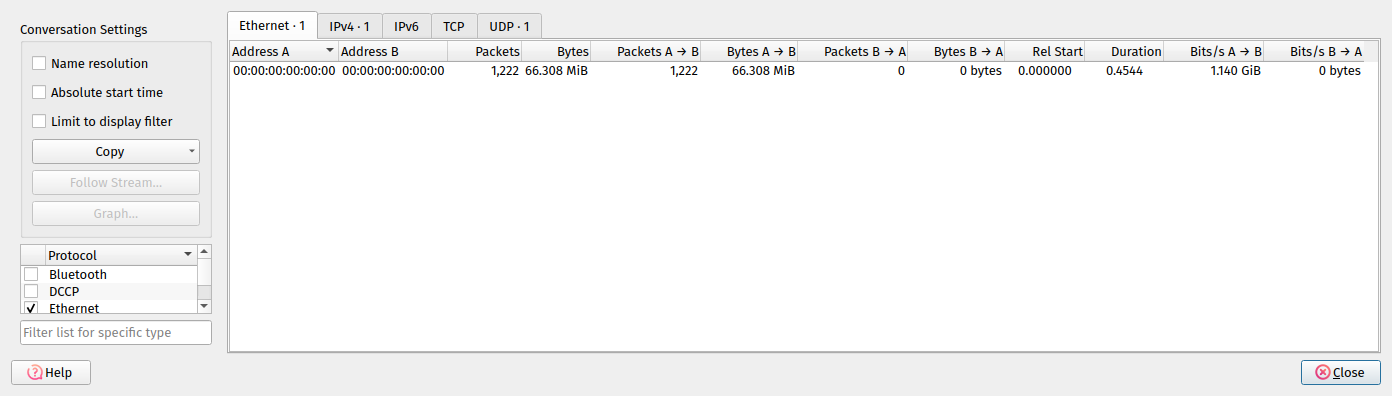
\includegraphics[width=\linewidth]{wireshark-conversations.png}
    \caption{Wireshark Conversations}
\end{figure}

\begin{figure}[h!]
    \centering
    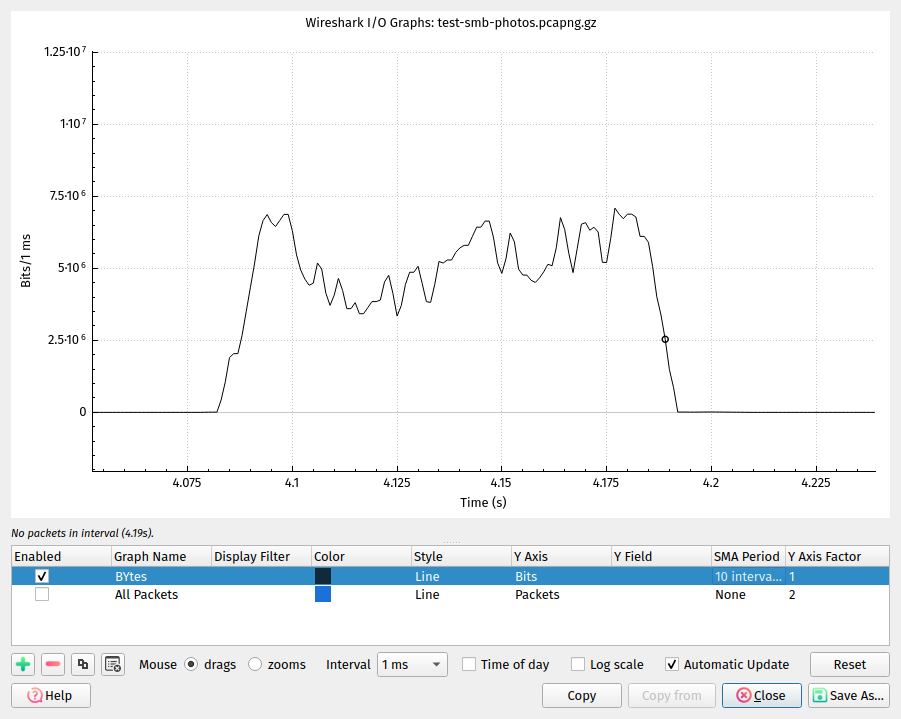
\includegraphics[width=0.7\linewidth]{wireshark-iograph.png}
    \caption{Wireshark IO Graph}
\end{figure}

\newpage

\section{Results}
\subsection*{Existing Solutions}
\begin{table}[h!]
	\caption{Existing Protocols Test Results}
	\label{tab:existing-protocols-test-results}
	\centering
	\begin{tabular}{l l l l l l}
		\textbf{Single}     &                      &                        &                         &                         &                      \\
		\textbf{}           & \textbf{Total Bytes} & \textbf{Total Packets} & \textbf{Transfer Speed} & \textbf{Overhead Bytes} & \textbf{Overhead \%} \\
		\hline
		\textbf{FTP}        & 2,015,995            & 188                    & 2.4Kbps                 & 15,995                  & 0.79\%               \\
		\hline
		\textbf{SMB}        & 2,049,153            & 323                    & 29.1Kbps                & 49,153                  & 2.40\%               \\
		\hline
		\textbf{RSYNC}      & 2,014,762            & 212                    & 263.5Kbps               & 14,762                  & 0.73\%               \\
		\hline
		                    &                      &                        &                         &                         &                      \\
		\textbf{Text}       &                      &                        &                         &                         &                      \\
		\textbf{}           & \textbf{Total Bytes} & \textbf{Total Packets} & \textbf{Transfer Speed} & \textbf{Overhead Bytes} & \textbf{Overhead \%} \\
		\hline
		\textbf{FTP}        & 136,196              & 661                    & 20.2Kbps                & 63,442                  & 46.58\%              \\
		\hline
		\textbf{SMB}        & 172,501              & 528                    & 151.0Kbps               & 99,747                  & 57.82\%              \\
		\hline
		\textbf{RSYNC}      & 77,101               & 42                     & 2.5Mbps                 & 4,347                   & 5.64\%               \\
		\hline
		                    &                      &                        &                         &                         &                      \\
		\textbf{Photos}     &                      &                        &                         &                         &                      \\
		\textbf{}           & \textbf{Total Bytes} & \textbf{Total Packets} & \textbf{Transfer Speed} & \textbf{Overhead Bytes} & \textbf{Overhead \%} \\
		\hline
		\textbf{FTP}        & 67,481,283           & 3,332                  & 78.0Mbps                & 239,590                 & 0.36\%               \\
		\hline
		\textbf{SMB}        & 67,551,796           & 2,879                  & 69.0Mbps                & 310,103                 & 0.46\%               \\
		\hline
		\textbf{RSYNC}      & 67,471,457           & 3,212                  & 1.0Gbps                 & 229,764                 & 0.34\%               \\
		\hline
		                    &                      &                        &                         &                         &                      \\
		\textbf{1KB Random} &                      &                        &                         &                         &                      \\
		\textbf{}           & \textbf{Total Bytes} & \textbf{Total Packets} & \textbf{Transfer Speed} & \textbf{Overhead Bytes} & \textbf{Overhead \%} \\
		\hline
		\textbf{FTP}        & 15,275,292           & 23,150                 & 1.1Mbps                 & 14,763,292              & 96.65\%              \\
		\hline
		\textbf{SMB}        & 2,945,640            & 11,194                 & 1.0Mbps                 & 2,433,640               & 82.62\%              \\
		\hline
		\textbf{RSYNC}      & 571,065              & 69                     & 36.6Mbps                & 59,065                  & 10.34\%              \\
		\hline
	\end{tabular}
\end{table}

\newpage

\subsection*{Prototypes}
\begin{table}[h!]
	\caption{Prototypes Test Results}
	\label{tab:prototypes-test-results}
	\centering
	\begin{tabular}{l l l l l l}
		\textbf{Single}     &                      &                        &                         &                         &                      \\
		\textbf{}           & \textbf{Total Bytes} & \textbf{Total Packets} & \textbf{Transfer Speed} & \textbf{Overhead Bytes} & \textbf{Overhead \%} \\
		\hline
		\textbf{One}        & 2002786              & 39                     & 8.0Gbps                 & 2,786                   & 0.14\%               \\
		\hline
		\textbf{Two}        & 2133076              & 45                     & 2.5Gbps                 & 133,076                 & 6.24\%               \\
		\hline
		\textbf{Three}      & 2197453              & 46                     & 5.8Gbps                 & 197,453                 & 8.99\%               \\
		\hline
		                    &                      &                        &                         &                         &                      \\
		\textbf{Text}       &                      &                        &                         &                         &                      \\
		\textbf{}           & \textbf{Total Bytes} & \textbf{Total Packets} & \textbf{Transfer Speed} & \textbf{Overhead Bytes} & \textbf{Overhead \%} \\
		\hline
		\textbf{One}        & 78,636               & 79                     & 163.0Mbps               & 5,882                   & 7.48\%               \\
		\hline
		\textbf{Two}        & 80,766               & 109                    & 17.5Mbps                & 8,012                   & 9.92\%               \\
		\hline
		\textbf{Three}      & 78,994               & 109                    & 210.0Mbps               & 6,240                   & 7.90\%               \\
		\hline
		                    &                      &                        &                         &                         &                      \\
		\textbf{Photos}     &                      &                        &                         &                         &                      \\
		\textbf{}           & \textbf{Total Bytes} & \textbf{Total Packets} & \textbf{Transfer Speed} & \textbf{Overhead Bytes} & \textbf{Overhead \%} \\
		\hline
		\textbf{One}        & 68,425,889           & 1,128                  & 1.9Gbps                 & 1,184,196               & 1.73\%               \\
		\hline
		\textbf{Two}        & 68,560,332           & 1,192                  & 225.9Mbps               & 1,318,639               & 1.92\%               \\
		\hline
		\textbf{Three}      & 69,529,440           & 1,222                  & 1.1Gbps                 & 2,287,747               & 3.29\%               \\
		\hline
		                    &                      &                        &                         &                         &                      \\
		\textbf{1KB Random} &                      &                        &                         &                         &                      \\
		\textbf{}           & \textbf{Total Bytes} & \textbf{Total Packets} & \textbf{Transfer Speed} & \textbf{Overhead Bytes} & \textbf{Overhead \%} \\
		\hline
		\textbf{One}        & 714,158              & 2,504                  & 46.0Mbps                & 202,158                 & 28.31\%              \\
		\hline
		\textbf{Two}        & 785,906              & 3,504                  & 4.7Mbps                 & 273,906                 & 34.85\%              \\
		\hline
		\textbf{Three}      & 728,846              & 3,504                  & 35.4Mbps                & 216,846                 & 29.75\%              \\
		\hline
	\end{tabular}
\end{table}
